This section describes the characterization of uncladded BCF-12 fibers from Saint-Gobain, which are the fibers selected for the TRITIUM experiment. These fibers are compared to single clad and multiclad BCF-12 fibers to quantify the influence of the clad in the relevant parameters of the scintillating fibers.

Although commercial clads are too thick for the TRITIUM experiment, a low thickness clad could be developed. For example, clads with a thickness of the order of tens of nanometers could be achieved by electrodeposition techniques. The difference between these three types of fibers is that uncladded fibers only consist of a polystyrene core with a refractive index of $1.60$ whereas single clad fibers have an acrylic clad (PMMA) of $30~\mu\meter$ thickness and a refractive index of $1.49$ and, multiclad fibers have a second fluor-acrylic clad of $10~\mu\meter$ thickness  and a refractive index of 1.42. The clad affects the photon collection efficiency of the fiber and prevents the fiber core from being damaged due to harsh environments.

%The first measurement that was made is the measurement of the diameter of the fiber. It is important because scintillating molecules are only present in the polystyrene core and we need to know whether the entire polystyrene core is the same size or not. Three different samples of each type of fiber were measured and the results are presented in Table \ ref {}.

%TABLAAA DIAMETROOOS

%Therefore, we can see that all fibers have the same external size, which means that the diameter of the polystyrene core is smaller for single clad fibers ($0.97~\mm$) and even smaller for multiclad fibers ($0.96~\mm$). It is an important result since...

This characterization was carried out for single scintillating fibers and consists of a comparative study of uncertainty in the fiber response that will affect to the tritium measurement made with the TRITIUM detector. In addition an estimation of the photon collection efficiency of the fibers types mentioned above was done. The magnitude employed for the characterization was the rate of photons reaching the active area of the photosensor with increasing light input at the entrance of the fiber. To measure this magnitude, a calibrated PMT (Hamamatsu R8520-06SEL) with $29.76\%$ quantum efficiency at $435~\nm$ was used. The PCB described in section \ref{subsubsec:PMTs} was used to switch the PMT internal gain off and mesure its photocurrent using a Picoammeter (Keithley 6487 picoammeter/voltage source). The photon rate was obtained from the current measurement using the equation \ref{eq:NumPhotonsFromIntensityPMT} with $QE=0.2976$ and $CE=1$. A simplified scheme of the setup is shown in Figure \ref{fig:SetUpFiberCharacterization}.

\begin{figure}[h]
\centering
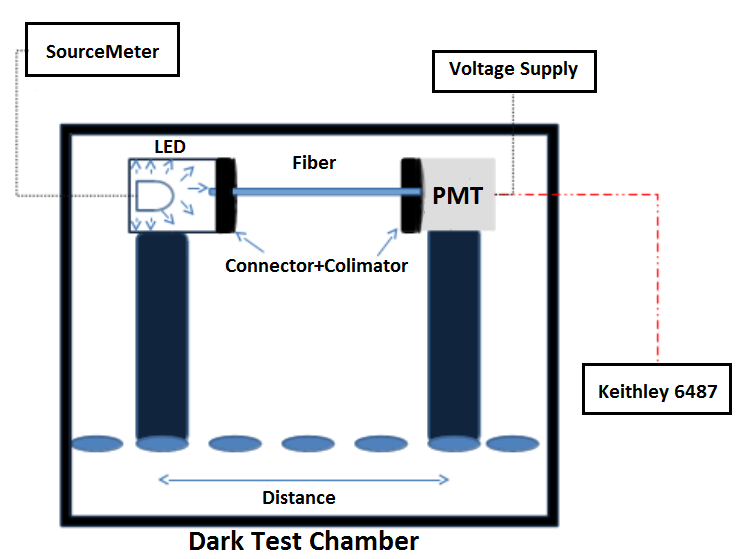
\includegraphics[scale=0.6]{4ResearchAndDevelopments/41Fibers/SetUp_Fiber_Characterization.png}
\caption{Setup used for fiber characterization.\label{fig:SetUpFiberCharacterization}}
\end{figure}

This setup consists of a home-made optical board, on which a LED and a the PMT are placed precisely in front of each other at an appropriate distance. A LED (LED435-03 from Roithner LaserTechnik Gmbh \cite{LEDRLT}), with an emission spectrum similar to that of the scintillating fibers, was used. The emission spectrum of the LED, given in Figure \ref{fig:LEDSpectrumTritium}, was experimentaly measured using a spectrometer and fitted to a Gaussian function. The LED emission peak is at $433.9~\nano\meter$ with a $\sigma$ of $7.85~\nm$. The LED is feeded in current mode to achieve a linear dependence on the light emision and the current used to feed it. The fiber of $20~\cm$ long was placed between the LED and the PMT, closely coupled to them at each of its end-surfaces, using optical grease \cite{OpticalGrease}. Two collimators were used to ensure that only photons emitted from the LED were detected by the PMT. Two conectors (FH-ST\footnote{FH-ST is a quick assembly connector for $1~\mm$ diameter plastic optical fiber, POF} connectors from RoHS company \cite{}) were used to fasten the fiber to the system. 

\begin{figure}[h]
\centering
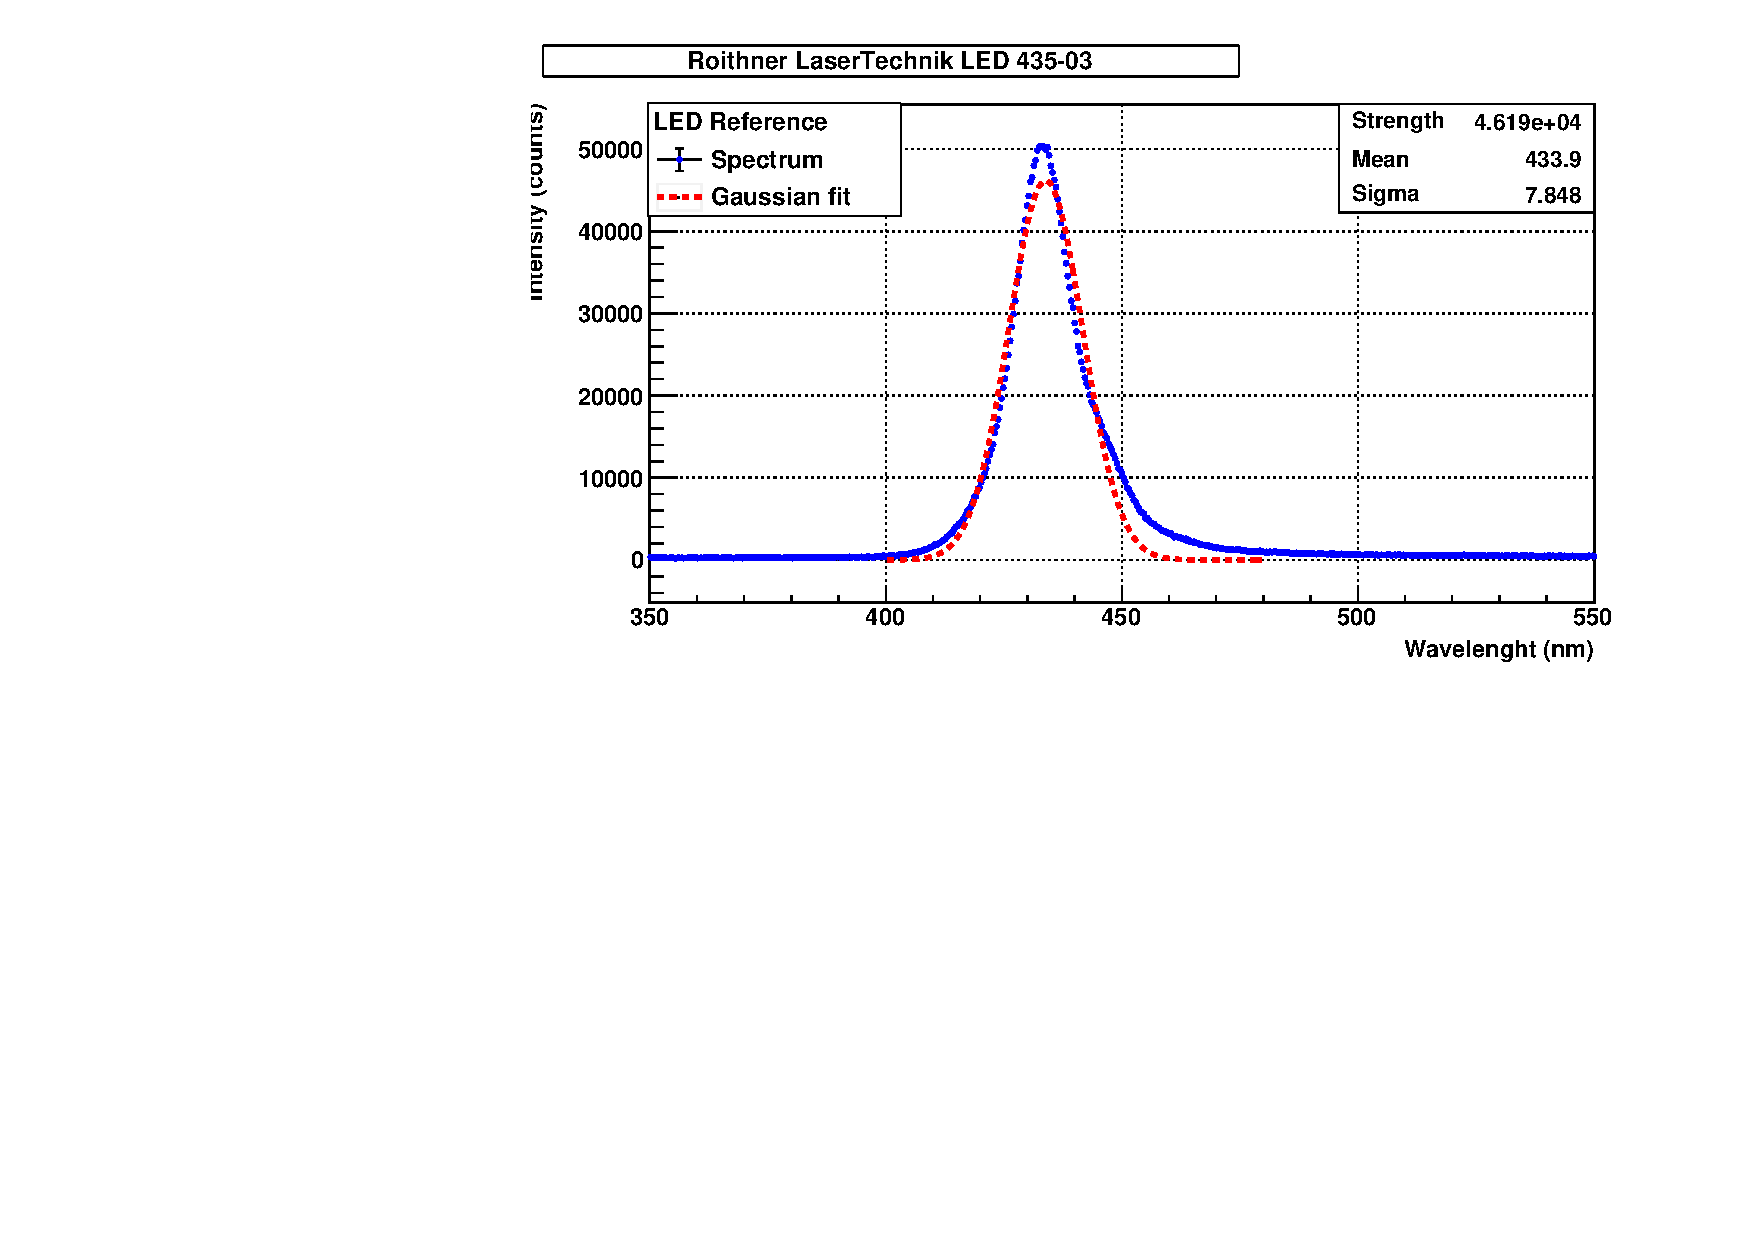
\includegraphics[scale=0.6]{4ResearchAndDevelopments/41Fibers/LED_TRITIUM_1_std.pdf}
\caption{Emission spectrum measured in the laboratory for the LED model 435-03 from Roithner LaserTechnik Gmbh Company.\label{fig:LEDSpectrumTritium}}
\end{figure}